\begin{center}
\begin{figure}[ht]
\begin{center}
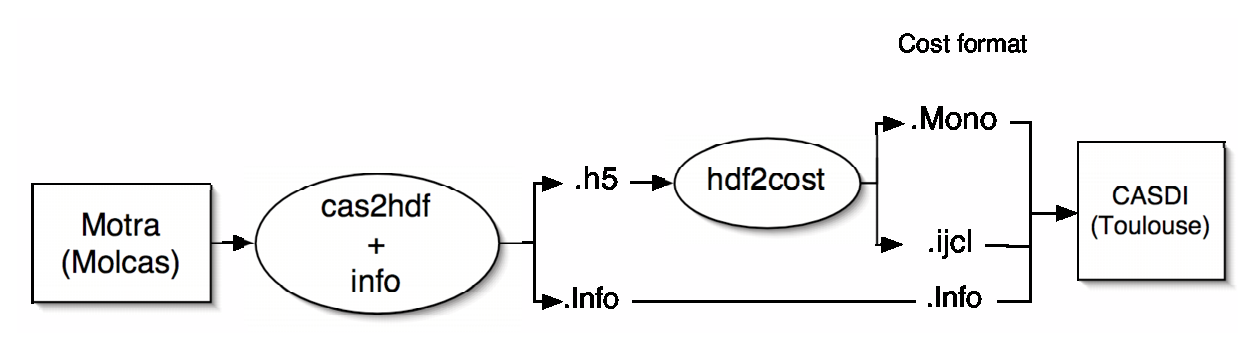
\includegraphics[width=10cm,keepaspectratio]{04_grid/images/q5cost-intermediate-gimped.eps}
\end{center}
\caption{\footnotesize A conservative solution. The \texttt{cas2hdf}
program produces the Q5Cost file, which is converted to the old COST format with
\texttt{hdf2cost}. The \texttt{.Info} file is used as a temporary
replacement of the XML file, and is provided by the \texttt{info}
program, directly interfaced with the \molcas suite. This solution does not
need changes in the CASDI code, and is therefore preferred in the initial
deployment. }
\label{fig:q5cost-intermediate}
\end{figure}
\end{center}
